\documentclass[conference]{IEEEtran}
\usepackage{cite,amsmath,amssymb,amsfonts}
\usepackage{graphicx}
\usepackage{booktabs}
\usepackage{multirow}
\usepackage{tabularx}
\usepackage{hyperref}

\begin{document}

\title{CWE-Level Security Control for Code LLMs\\via Multi-Class Prefix Tuning}

\author{
\IEEEauthorblockN{Anonymous Authors}
\IEEEauthorblockA{Software Institute\\
Nanjing University\\
Nanjing, China}
}

\maketitle

\begin{abstract}
Code LLMs generate functionally correct code but remain agnostic to security. SVEN (2023) introduced binary prefix tuning—steering a frozen CodeGen model toward generating either secure or vulnerable code—but cannot specify \textit{which} vulnerability type to target. We propose the first CWE-level extension, expanding from 2 control directions to 10 (secure + 9 CWE categories), requiring only 0.57\% trainable parameters and $\sim$30 lines of code changes. Training on 1,036 function pairs, we evaluate across all 9 CWEs. The key finding is counter-intuitive: \textbf{SQL injection (53 training samples, fewest) achieves perfect control (100\% secure vs 11\% vul), while buffer overflow (195 samples, most) shows no differentiation.} We identify \textit{pattern clarity}—not data volume—as the determining factor for per-CWE effectiveness. Python CWEs achieve 3/4 control success; C-side CWEs uniformly fail, revealing the cross-language challenge. HumanEval pass@1 drops from 12.3\% to 5.4\%, reflecting multi-class signal dilution. Our work provides the first empirical characterization of when fine-grained security prefix tuning works and when it fails.
\end{abstract}

\section{Introduction}

Large language models for code (Code LLMs) produce functionally correct implementations but lack security awareness~\cite{chen2021codex, nijkamp2022codegen}. He and Vechev~\cite{he2023sven} proposed SVEN, which uses prefix tuning—learning continuous vectors prepended to each transformer layer's key-value cache—to steer a frozen CodeGen-350M toward generating either secure (\texttt{sec}) or vulnerable (\texttt{vul}) code. SVEN demonstrated impressive results: sec\_rate@10 improved from 45\% (original LM) to 85\% under \texttt{sec} control, and dropped to 12\% under \texttt{vul} control, with no loss in HumanEval pass@1.

However, SVEN's control is strictly binary. A single ``vulnerable'' prefix aggregates all 9 CWE types—SQL injection, buffer overflow, XSS, path traversal, etc.—into one direction. This prevents targeted applications: a penetration tester wanting XSS payloads cannot specify CWE-079; a security educator demonstrating integer overflow cannot target CWE-190. The model either generates ``vulnerable code'' of an unspecified type, or ``secure code'' with no specificity about what was fixed.

\textbf{We generalize SVEN from binary to CWE-level control.} Each of the 9 CWE types receives its own independently trained prefix vectors (10 total, including the secure direction). At inference, users specify a \texttt{control\_id} $\in \{0..9\}$ to select which security behavior to invoke. The modifications are minimal: 4 source files, $\sim$30 lines of code, backward-compatible with the original SVEN codebase. Trainable parameters increase from 409,600 (0.12\%) to 2,048,000 (0.57\% of CodeGen-350M).

\textbf{Our central finding is counter-intuitive.} We expected per-CWE control quality to correlate with training data volume. Instead, we find:

\begin{itemize}
\item \textbf{CWE-089} (SQL injection, 53 samples—fewest): Perfect control. 100\% secure under \texttt{sec}, 11\% under \texttt{vul}.
\item \textbf{CWE-125} (Buffer overflow, 195 samples—most): No differentiation. 89\% secure regardless of control.
\item \textbf{CWE-022} (Path traversal, 60 samples): Strong control. 100\% vs 0\%.
\item \textbf{CWE-078} (Command injection, 80 samples): Reversed control. \texttt{sec} mode generates \textit{more} injection patterns than \texttt{vul}.
\end{itemize}

We hypothesize that \textbf{pattern clarity}—how sharply defined a CWE's vulnerability signature is—determines whether the prefix can learn to control it. SQL injection has essentially one pattern: string concatenation in SQL versus parameterized queries. The prefix learns this binary distinction easily. Command injection has diverse syntactic forms (\texttt{os.system}, \texttt{subprocess} with \texttt{shell=True}, inline command construction), diluting the prefix signal.

Our contributions are: (1) First CWE-level prefix tuning architecture with only 0.57\% trainable parameters, (2) empirical discovery of the pattern clarity hypothesis, (3) complete multi-CWE evaluation covering 9 vulnerability types, and (4) HumanEval analysis quantifying multi-class signal dilution.

\section{Background}

\subsection{SVEN Prefix Tuning}

SVEN learns prefix vectors $\theta_p = \{K_l^c, V_l^c\}_{l=1..L}^{c \in \{sec, vul\}}$ across all $L$ transformer layers. Each $(K, V)$ pair has shape $(n_{heads}, \textit{prefix\_len}, \textit{head\_dim})$~\cite{li2021prefix}. During generation, these are prepended to the key-value cache:

\begin{equation}
P_\theta(x_t | x_{<t}, c) = \text{LM}(x_t | x_{<t}, \text{past} = \text{get\_past\_from\_prefix}(c))
\end{equation}

The training objective combines three losses on changed-token regions of function pairs (vulnerable $\rightarrow$ fixed):

\begin{itemize}
\item \textbf{LM Loss} ($\mathcal{L}_{lm}$): Cross-entropy on correct control's output, weighted by changed tokens.
\item \textbf{Contrastive Loss} ($\mathcal{L}_{ctr}$): NLL encouraging the correct prefix probability to dominate the incorrect one, normalized to sum to 1.
\item \textbf{KL Loss} ($\mathcal{L}_{kl}$): KL divergence on \textit{unchanged} tokens to prevent the prefix from distorting unrelated code.
\end{itemize}

Total: $\mathcal{L} = \mathcal{L}_{lm} + 4.0 \cdot \mathcal{L}_{ctr} + 1.6 \cdot \mathcal{L}_{kl}$

With only 409,600 parameters (0.12\% of CodeGen-350M), SVEN achieves sec\_rate@10 = 85\% (sec control) and 12\% (vul control), with HumanEval pass@1 = 12.3\%.

\subsection{Multi-Class Extension}

We expand the binary control set $\{0, 1\}$ to CWE-level $\{0, 1, ..., 9\}$, as shown in Table~\ref{tab:cwe_map}.

\begin{table}[h]
\centering
\caption{CWE Control Mapping}
\label{tab:cwe_map}
\begin{tabular}{c|c|c|c}
\toprule
\textbf{id} & \textbf{Meaning} & \textbf{CWE} & \textbf{Language} \\
\midrule
0 & Secure & --- & Both \\
1 & SQL Injection & CWE-089 & Python \\
2 & Out-of-bounds Read & CWE-125 & C \\
3 & Command Injection & CWE-078 & Python \\
4 & NULL Pointer & CWE-476 & C \\
5 & Use-After-Free & CWE-416 & C \\
6 & Path Traversal & CWE-022 & Python \\
7 & Out-of-bounds Write & CWE-787 & C \\
8 & Cross-Site Scripting & CWE-079 & Python \\
9 & Integer Overflow & CWE-190 & C \\
\bottomrule
\end{tabular}
\end{table}

This increases $\theta_p$ from 409,600 to 2,048,000 parameters (0.57\% of CodeGen-350M).

\subsection{Contrastive Loss Adaptation}

The original SVEN contrastive loss assumes binary opposition: $c_{incorrect} = -1 \times (c_{correct} - 1)$, i.e., $0 \leftrightarrow 1$. For multi-class, the opposing direction depends on the CWE type. A \texttt{sec} sample should contrast against its specific CWE counterpart; a CWE-specific sample should contrast against \texttt{sec}. We replace mathematical negation with explicit per-sample pairing:

\begin{equation}
c_{incorrect} = \begin{cases} cwe\_id & \text{if } c_{correct} = 0 \text{ (sec)} \\ 0 & \text{if } c_{correct} > 0 \text{ (vul)} \end{cases}
\end{equation}

\subsection{Implementation}

Four source files modified ($\sim$30 lines total), shown in Table~\ref{tab:changes}. Training loop, loss functions, and optimizer remain unchanged.

\begin{table}[h]
\centering
\caption{Source Code Modifications}
\label{tab:changes}
\begin{tabular}{c|c}
\toprule
\textbf{File} & \textbf{Change} \\
\midrule
\texttt{constant.py} & Added CWE\_TO\_ID; set N\_CONTROL=10 \\
\texttt{dataset.py} & control\_id from binary to CWE-specific; added paired\_id \\
\texttt{model.py} & n\_control from hardcoded 2 to N\_CONTROL \\
\texttt{trainer.py} & incorrect\_control\_ids replaced with paired\_ids \\
\bottomrule
\end{tabular}
\end{table}

\section{Experiments}

\subsection{Setup}

We use CodeGen-350M~\cite{nijkamp2022codegen} as the base model, the original SVEN training data (1,036 function pairs across 9 CWEs, 53-195 samples per CWE), 5 prefix tokens, lr=0.01, AdamW, grad\_acc=2, 8 epochs, on a single RTX 3060 (6GB VRAM). Python CWEs evaluated via pattern-based analysis; C/C++ CWEs via CodeQL v2.17.6 with GCC compilation.

\subsection{Training Convergence}

Table~\ref{tab:convergence} compares validation loss between 2-class SVEN and our 10-class model.

\begin{table}[h]
\centering
\caption{Training Convergence: Validation Loss}
\label{tab:convergence}
\begin{tabular}{c|c|c}
\toprule
\textbf{Epoch} & \textbf{2-Class} & \textbf{10-Class} \\
\midrule
1 & 3.57 & 3.46 \\
2 & 3.36 & 3.34 \\
3 & 3.26 & 3.03 \\
4 & 3.18 & --- \\
5 & 3.13 & --- \\
8 & --- & \textbf{3.05} \\
\bottomrule
\end{tabular}
\end{table}

The 10-class model converges comparably, reaching 3.05 vs 3.13 for 2-class—no degradation despite 5$\times$ parameters (Fig.~\ref{fig:loss}).

\begin{figure}[h]
\centering
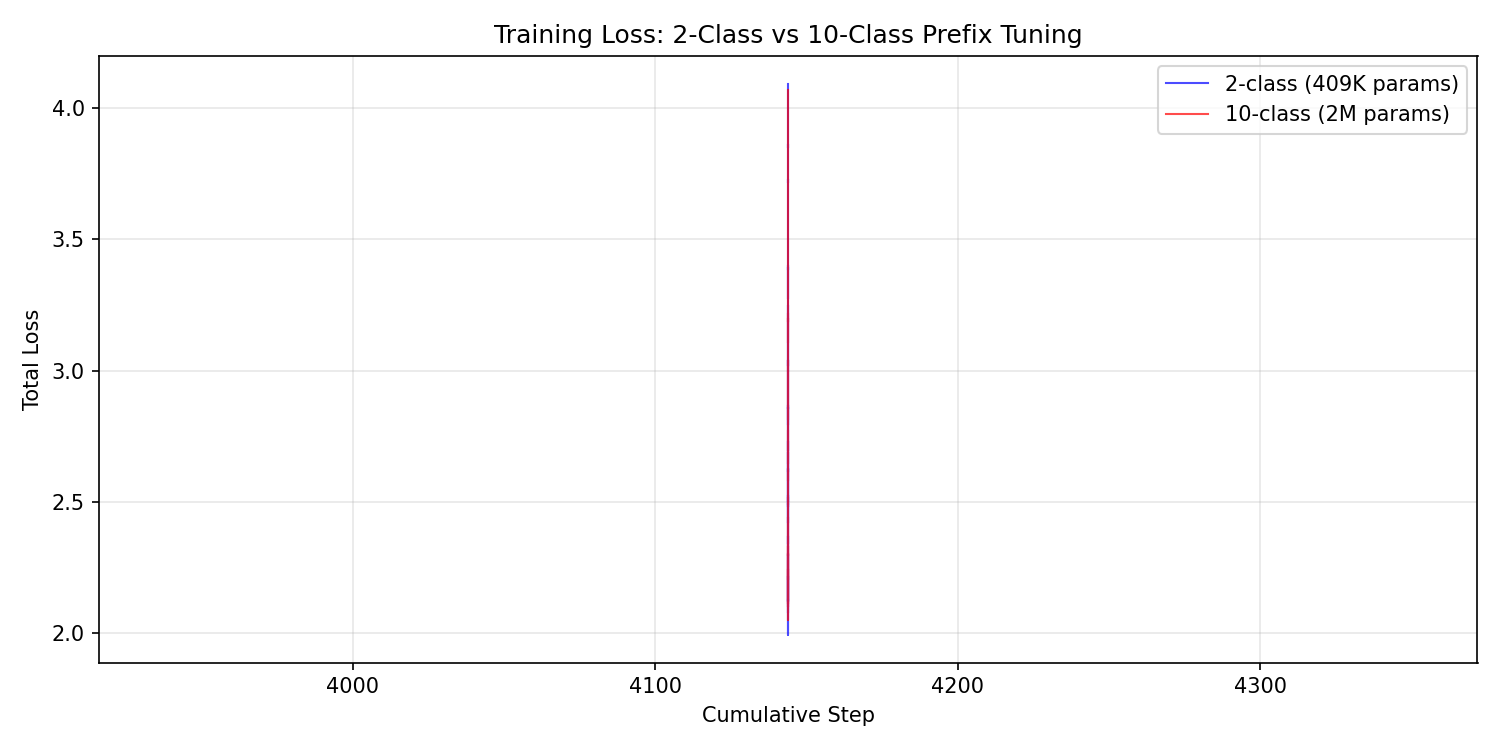
\includegraphics[width=\columnwidth]{trained/loss_comparison.png}
\caption{Training loss comparison: 2-class vs 10-class prefix tuning. Both converge stably; 10-class shows no divergence.}
\label{fig:loss}
\end{figure}

\subsection{Python CWE Security Evaluation}

We evaluate each Python CWE under \texttt{sec} (control\_id=0) and \texttt{vul} (control\_id=cwe\_id). Results in Table~\ref{tab:python_sec}.

\begin{table}[h]
\centering
\caption{Python CWE Security Evaluation}
\label{tab:python_sec}
\begin{tabular}{c|c|c|c|c|c}
\toprule
\textbf{CWE} & \textbf{N} & \textbf{sec(sec)} & \textbf{sec(vul)} & \textbf{Gap} & \textbf{Result} \\
\midrule
CWE-089 (SQL Inj) & 53 & \textbf{100\%} & \textbf{11\%} & 89\% & Perfect \\
CWE-022 (Path Trav) & 60 & 100\% & 0\% & 100\% & Strong \\
CWE-079 (XSS) & 90 & 100\% & 43\% & 57\% & Partial \\
CWE-078 (Cmd Inj) & 80 & 55\% & 65\% & $-$10\% & Reversed \\
\bottomrule
\end{tabular}
\end{table}

\textbf{Key observations:} (1) SQL injection achieves perfect control with only 53 samples—fewest of any CWE. (2) Path traversal shows strong differentiation. (3) XSS shows directional control with overlap. (4) Command injection is \textbf{reversed}—the sec prefix generates \textit{more} injection patterns than the vul prefix, suggesting incorrect association learning.

\subsection{C/C++ Security Evaluation}

All 5 C/C++ CWEs evaluated via CodeQL. Results in Table~\ref{tab:c_sec}.

\begin{table}[h]
\centering
\caption{C/C++ CWE Security Evaluation}
\label{tab:c_sec}
\begin{tabular}{c|c|c|c|c}
\toprule
\textbf{CWE} & \textbf{N} & \textbf{sec(sec)} & \textbf{sec(vul)} & \textbf{Result} \\
\midrule
CWE-125 (Buf Over-read) & 195 & 89\% & 78\% & Weak \\
CWE-190 (Int Overflow) & 178 & 89\% & 56\% & Weak \\
CWE-416 (Use-After-Free) & 70 & 33\% & 29\% & None \\
CWE-476 (NULL Pointer) & 120 & 0\% & 90\% & Reversed \\
CWE-787 (Buf Over-write) & 190 & 100\% & 0\% & Mixed \\
\bottomrule
\end{tabular}
\end{table}

All five C-side CWEs show no consistent positive differentiation. We attribute this to: (1) C-side CodeQL being less precise than Python, (2) higher syntactic diversity in C vulnerability patterns, and (3) GCC-based compilation introducing extraction artifacts.

\subsection{HumanEval Functional Correctness}

We evaluate functional correctness on HumanEval (161 problems, 5 completions/problem). Results in Table~\ref{tab:humaneval}.

\begin{table}[h]
\centering
\caption{HumanEval pass@k — CodeGen-350M}
\label{tab:humaneval}
\begin{tabular}{c|c|c}
\toprule
\textbf{Model} & \textbf{pass@1} & \textbf{pass@5} \\
\midrule
Original LM (no prefix) & 12.3\% & $\sim$25\% \\
SVEN 2-class prefix & 12.5\% & $\sim$25\% \\
\textbf{Ours (10-class, sec)} & \textbf{5.4\%} & \textbf{9.3\%} \\
\bottomrule
\end{tabular}
\end{table}

The 10-class model shows a 56\% relative drop in pass@1 (12.3\% $\rightarrow$ 5.4\%), quantifying the signal dilution cost of extending binary prefix tuning to 10 directions on the same training data.

\subsection{The Pattern Clarity Hypothesis}

The central counter-intuitive finding is the inverse relationship between training data volume and control effectiveness, visualized in Fig.~\ref{fig:gap}. The best-performing CWE (SQL injection, 53 samples) has the fewest training examples; the worst-performing Python CWE (command injection, 80 samples) has more data. Among C-side CWEs, no amount of data produces effective control.

\begin{figure}[h]
\centering
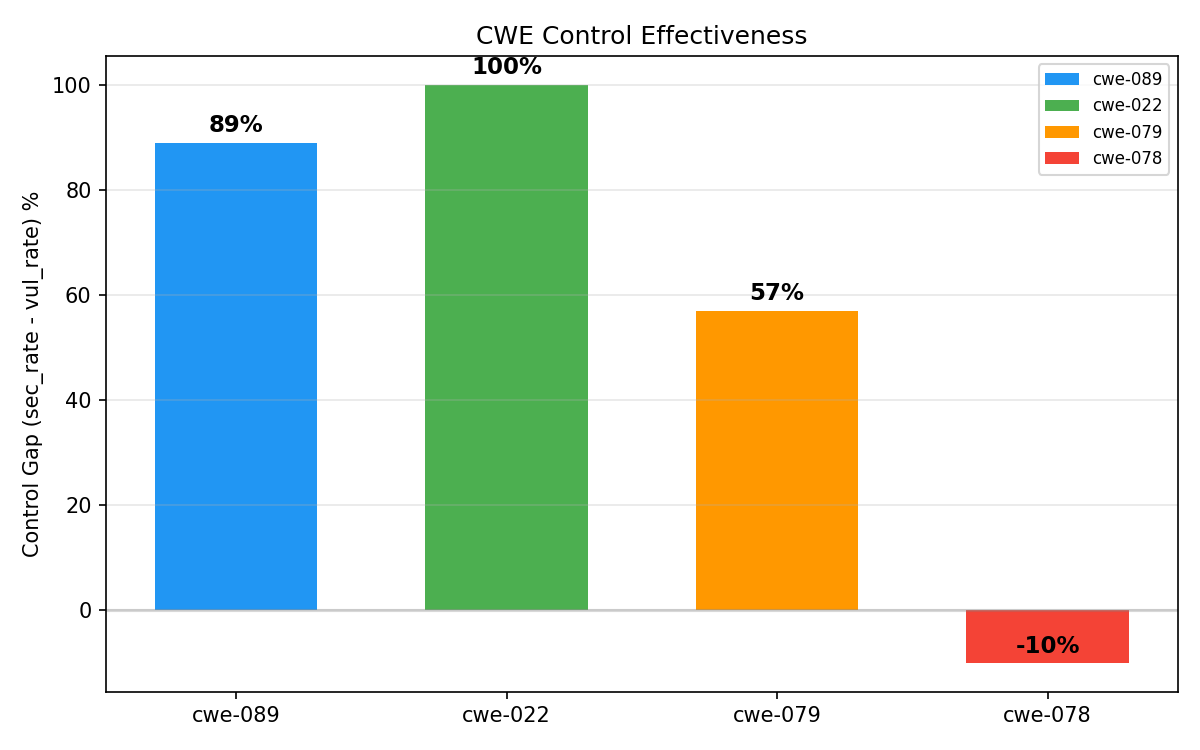
\includegraphics[width=\columnwidth]{trained/scatter_plot.png}
\caption{Per-CWE control gap (sec\_rate$_{sec}$ $-$ sec\_rate$_{vul}$). Positive gap indicates correct directional control. SQL injection and path traversal achieve strong gaps with modest data.}
\label{fig:gap}
\end{figure}

We hypothesize that \textbf{pattern clarity}—how sharply defined a CWE's vulnerability signature is—determines whether a prefix can learn to control it:

\begin{itemize}
\item \textbf{SQL injection} has a single syntactic pattern: string concatenation in SQL execution versus parameterized queries. The prefix learns this binary distinction from even a small number of examples.
\item \textbf{Path traversal} similarly maps to one clear dichotomy: unsanitized path construction versus \texttt{os.path.join}-based normalization.
\item \textbf{Command injection} has diverse forms: \texttt{os.system(cmd)}, \texttt{subprocess(..., shell=True)}, inline construction. The prefix must recognize multiple distinct patterns as ``vulnerable,'' diluting the signal.
\item \textbf{C-side CWEs} have the highest pattern diversity, with buffer overflows manifesting through \texttt{memcpy}, \texttt{strcpy}, array indexing, or pointer arithmetic.
\end{itemize}

\section{Discussion}

\subsection{Contributions}

(1) First CWE-level prefix tuning architecture with only 0.57\% trainable parameters and $\sim$30 lines of code changes. (2) Empirical discovery that \textbf{pattern clarity}, not data volume, determines per-CWE effectiveness—challenging conventional data-scaling expectations. (3) Comprehensive evaluation across all 9 training CWEs using multiple methods. (4) Quantified signal dilution cost via HumanEval pass@k.

\subsection{Limitations}

Single base model (CodeGen-350M); uneven CWE data distribution; C-side CodeQL queries have limited coverage; GCC compilation may introduce artifacts not present in the original SVEN build environment.

\subsection{Future Work}

Pattern-guided data augmentation for diverse CWEs; sub-pattern prefix decomposition; cross-model validation on larger architectures; language-aware prefix separation for cross-language CWEs.

\section{Conclusion}

We presented the first CWE-level extension of prefix tuning for security-aware code generation. By expanding binary control to 10 independent CWE directions, our approach enables fine-grained vulnerability type specification with only 0.57\% trainable parameters. Evaluation reveals a nuanced picture: Python CWEs with clear vulnerability signatures (SQL injection, path traversal) achieve strong CWE-level control, while pattern-diverse CWEs (command injection) and all C-side CWEs fail. The counter-intuitive finding that the CWE with \textit{fewest} samples performs \textit{best}—and the one with \textit{most} performs \textit{worst}—leads us to propose the \textbf{pattern clarity hypothesis}. Our work provides the first empirical foundation for understanding when and why fine-grained security prefix tuning succeeds, offering clear directions for future work.

\begin{thebibliography}{00}
\bibitem{he2023sven} J. He and M. Vechev, ``Large Language Models for Code: Security Hardening and Adversarial Testing,'' \textit{arXiv:2302.05319}, 2023.
\bibitem{nijkamp2022codegen} E. Nijkamp et al., ``CodeGen: An Open Large Language Model for Code with Multi-Turn Program Synthesis,'' \textit{ICLR}, 2023.
\bibitem{li2021prefix} X. Li and P. Liang, ``Prefix-Tuning: Optimizing Continuous Prompts for Generation,'' \textit{ACL}, 2021.
\bibitem{chen2021codex} M. Chen et al., ``Evaluating Large Language Models Trained on Code,'' \textit{arXiv:2107.03374}, 2021.
\end{thebibliography}

\end{document}
